\section{Lecture 9: Dynamic Games}
\newsection
There are different game types. Static or Dynamic, Complete info or incomplete info, perfect info and imperfect info.

\definition{Dynamic Game}{
 Everybody knows what a dynamic game is. You know it when you see it.
}
\begin{aexample}{Entry Game}{}
    A company (A) can enter the market or decide not to enter the market. Another company (B) is incumbent (already in the market) and can decide to cut or hold prices. The payoff matrix is as follows.
    \begin{center}
        \begin{tabular}{|c|c c|}
            \hline
            A\textbackslash B & cut & hold\\
            \hline
            Don't Enter & (0,2) & (0,3)   \\
            \hline Enter & (-1,1),& (1,1) \\  \hline  
        \end{tabular}
    \end{center}
    The Nash equilibrium is Enter and Hold.
\end{aexample}
However, we can model the game using an extensive form representation. Each B represents a subgame. There are two subgames depending on A's action.
\begin{center}
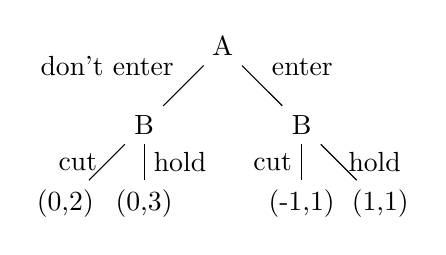
\begin{tikzpicture}
    \node (A) at (0,0){A};
    \node(B) at (-1,-1) {B};
    \node(C) at (1,-1) {B};
    \node(D) at (-2,-2) {(0,2)};
    \node(E) at (-1,-2) {(0,3)};
    \node(F) at (1,-2) {(-1,1)};
    \node(G) at (2,-2) {(1,1)};
    \draw (A) edge  node[midway, above left]{don't enter}(B);
    \draw (A) edge  node[midway, above right]{enter}(C);
    \draw (B) edge  node[midway,  left]{cut}(D);
    \draw (B) edge node[midway,  right]{hold} (E) ;
    \draw (C) edge  node[midway,  left]{cut}(F);
    \draw (C) edge  node[midway,  right]{hold}(G);
\end{tikzpicture}\end{center}
Therefore, we can expand the strategy set of B to be 
\begin{center}
    \begin{tabular}{|c|c c c c|}
        \hline
        A\textbackslash B & (cut, cut) & (cut, hold) &(hold, cut) & (hold, hold) \\
        \hline
        Don't Enter & (0,2) &(0,2)&(0,3)& (0,3)   \\
        \hline Enter & (-1,1),& (1,1)  & (-1,1),& (1,1) \\  \hline  
    \end{tabular}
\end{center}
Therefore, we get a Nash equilibria of (enter, (cut,hold)), (enter, (hold,hold)), (don't enter, (hold,cut)).

However, the first equilibrium is a bit weird. This is because we are implying that B will cut if A doesn't enter. We call this equilibrium \textbf{not sequentially rational}.
\definition{Sequential rationality}{
    A pure strategy Nash equilibrium is said to be \textbf{sequentially rational}, or a \textbf{subgame perfect Nash equilibrium} if the agents' strategies continue to be a Nash equilibrium in every sub game.

}

We can check this using a backward induction algorithm. 
We first consider the strategies B can have at each subgame. If A doesnt enter, then B plays hold. If A enters, it does not matter which one. Now we propagate backwards. If B plays (hold,cut), then A's decision tree is 
\begin{center}
    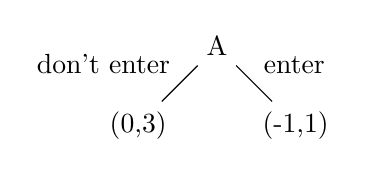
\begin{tikzpicture}
        \node (A) at (0,0){A};
        \node(B) at (-1,-1) {(0,3)};
        \node(C) at (1,-1) {(-1,1)};
        \draw (A) edge  node[midway, above left]{don't enter}(B);
        \draw (A) edge  node[midway, above right]{enter}(C);
    \end{tikzpicture}\end{center}
So (don't enter, (hold,cut)) is a subgame perfect Nash equilibrium.

\begin{atheorem}{}{}
    For a finite dynamic game, the backwards induction algorithm yields exactly all the subgame perfect Nash equilibria.
\end{atheorem}
\begin{aexample}{}{}
    Return to example \ref{ex:attackdefend}.
    \begin{center}
        \begin{tabular}{|c|c c|} 
            \hline
            Attacker\textbackslash User & A&B \\ 
            \hline
            A & (1,0) & (0,1)\\ 
            \hline
            B & (0,1)&(1,0)\\
            \hline
        \end{tabular}
    \end{center}
    We can change this into an extensive form - 
    \begin{center}
        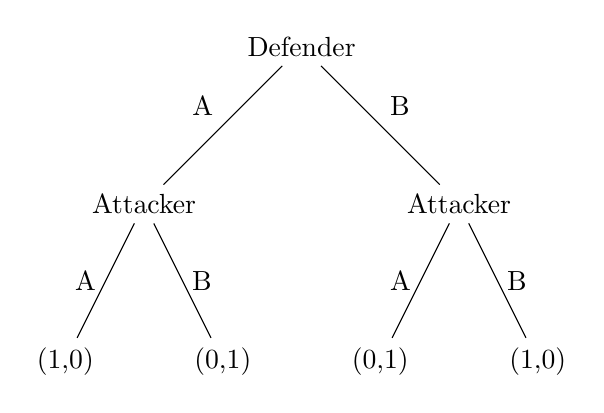
\begin{tikzpicture}
            \node (A) at (0,0){Defender};
            \node(B) at (-2,-2) {Attacker};
            \node(C) at (2,-2) {Attacker};
            \node(D) at (-3,-4) {(1,0)};
            \node(E) at (-1,-4) {(0,1)};
            \node(F) at (1,-4) {(0,1)};
            \node(G) at (3,-4) {(1,0)};
            \draw (A) edge  node[midway, above left]{A}(B);
            \draw (A) edge  node[midway, above right]{B}(C);
            \draw (B) edge  node[midway,  left]{A}(D);
            \draw (B) edge node[midway,  right]{B} (E) ;
            \draw (C) edge  node[midway,  left]{A}(F);
            \draw (C) edge  node[midway,  right]{B}(G);
        \end{tikzpicture}\end{center}
    It is obvious that the attacker has the advantage by choosing the strategy (A,B). The attacker is said to have a \textbf{second mover advantage} as the follower.
\end{aexample}
\begin{aexample}{Stackelberg Competition}{}
    Consider the sequential version of the \hyperref[ex:cournot]{Cournot competition}. Suppose in addition that $c_1=c_2=c\in [0,1]$. Now, let firm 1 plays first, then firm 2.
    Then firm 2's strategy is just to play $B_2(q_1) =  \max\{(1-q_1-c)/2,0\}.$ Naturally we can define $q_2= q_2(q_1)= B_2(q_1).$
    Then $q_1$ is the best response to $q_2$ strategy\[
    B_1(q_2) = \arg\max_{q_1\geq 0} (1-q_1-q_2(q_1))-cq_1. 
\]
solving this yields\[
q_1^*=\frac{1-c}{2},q_2^*=\frac{1-c}{4}.\]
\end{aexample}
Let us compare this to the Nash equilibirum of the static Cournot competition $((1-c)/3,(1-c)/3)$. 
The total quantity produced is \[
3\frac{(1-c)}{4} > 2\frac{(1-c)}{3},
\]
this is good for the consumer because the prices are lower. 
Firm one profits \[
\frac{1-c}{8} > \frac{1-c}{9}.
\]
Form two profits \[
\frac{1-c}{16} > \frac{1-c}{9}.
\]
This game has a first mover advantage. 

\textcolor{red}{TODO: too much work to draw these trees... but you probably understand the concept so whatever}
\begin{aexample}{Three player game}{}
    The outcome at the subgame perfect Nash equilibrium is R,L,R, with a strategy \[
    \{(R,L,(R,R,L))\}.
    \]
\end{aexample}

\begin{aexample}{}{}
    \begin{center}
        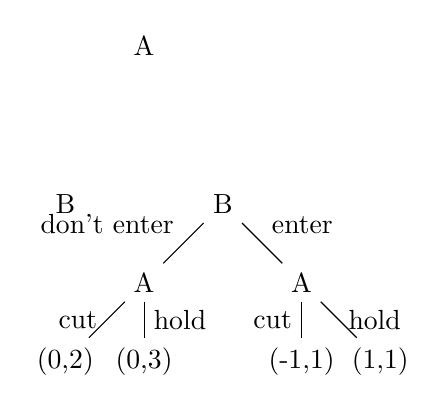
\begin{tikzpicture}
            \node(top) at (-1,2){A};
            \node (ll) at (-2,0) {B};
            \node (A) at (0,0){B};
            \node(B) at (-1,-1) {A};
            \node(C) at (1,-1) {A};
            \node(D) at (-2,-2) {(0,2)};
            \node(E) at (-1,-2) {(0,3)};
            \node(F) at (1,-2) {(-1,1)};
            \node(G) at (2,-2) {(1,1)};
            \draw (A) edge  node[midway, above left]{don't enter}(B);
            \draw (A) edge  node[midway, above right]{enter}(C);
            \draw (B) edge  node[midway,  left]{cut}(D);
            \draw (B) edge node[midway,  right]{hold} (E) ;
            \draw (C) edge  node[midway,  left]{cut}(F);
            \draw (C) edge  node[midway,  right]{hold}(G);
        \end{tikzpicture}\end{center}
\end{aexample}